\documentclass[border=10pt]{standalone}
\usepackage{pgfplots}
\pgfplotsset{compat=1.17}
\begin{document}
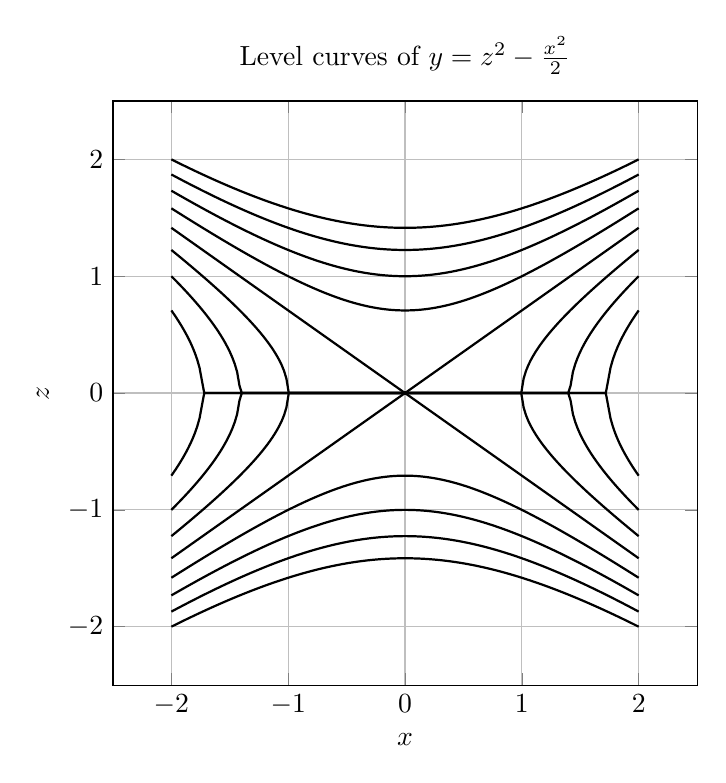
\begin{tikzpicture}
\begin{axis}[
    xlabel={$x$}, ylabel={$z$},
    title={Level curves of $y=z^2-\frac{x^2}{2}$},
    width=9cm,
    height=9cm,
    axis equal,
    xmin=-2.5, xmax=2.5,
    ymin=-2.5, ymax=2.5,
    grid=major,
    colormap/viridis,
    legend pos=south east
]
\foreach \c in {-1.5,-1,-0.5,0,0.5,1,1.5,2}{
    \addplot[thick, domain=-2:2, samples=200, forget plot] ({x}, {sqrt(max(\c+x^2/2,0))});
    \addplot[thick, domain=-2:2, samples=200, forget plot] ({x}, {-sqrt(max(\c+x^2/2,0))});
}
\end{axis}
\end{tikzpicture}
\end{document}
